% PDF MUST BE TITLED UGECEAnishGoyal2024.pdf
% All red text in the resulting paper (if any) is TO DO by Anish. 
% All blue text in the resulting paper (if any) is TO DO for Dr. Taheri 

%========================= Preamble ========================
\documentclass[pra, superscriptaddress]{revtex4-2}
\usepackage{graphicx}
\usepackage{wrapfig}
\usepackage{amsmath}
\usepackage{lipsum}
\usepackage{xcolor}
\usepackage{tikz}

\begin{document}

%========================= Metadata =========================

% Title
\title{ConcreteNet: A Deep Convolutional Neural Network for Deformity \\ Detection and Classification in Ground-Penetrating Radar Images}

% Date
\date{\today}

% Student
\author{Anish Goyal}
\affiliation{Freshman, Eagle ID 901414697, Department of Electrical and Computer Engineering, Georgia Southern University, Statesboro, GA 30460-8031, USA}

% Faculty mentor
\author{Hossein Taheri}
\affiliation{Associate Professor, Department of Manufacturing Engineering, Georgia Southern University, Statesboro, GA 30460-8031, USA}

% Abstract
\begin{abstract}
\vspace{2em}
\section*{ABSTRACT}

% \begin{description}
% \item[Background] The integrity of modern concrete structures is critical for public safety and infrastructure longevity. Current non-destructive testing (NDT) methods, particularly ground-penetrating radar (GPR), provide crucial insights into the internal conditions of concrete. However, traditional analysis techniques struggle with radargram data due to its complexity and noise, highlighting the need for advanced automated systems to detect structural anomalies more accurately.

% \item[Purpose] In this research project, we propose ConcreteNet, a discriminative convolutional neural network (CNN) architecture optimized for image classification on GPR radargrams, utilizing the "Network in Network" approach to capture and process complex patterns. AlexNet will serve as the base architecture for the initial model.

% \item[Method] The data for this study will be gathered from two main sources: (1) scans from the Georgia Southern Engineering Research Building (ERB), chosen for its recent construction date and contemporary design, and (2) pre-existing GPR data from the Georgia Department of Transportation. ConcreteNet will be trained and validated on this data to ensure robust performance in detecting structural anomalies.

% \item[Future Work] Potential extensions for this project include the use of autoencoders for unsupervised feature learning and the incorporation of recurrent neural networks (RNNs) with Long Short-Term Memory (LSTM) layers to improve classification accuracy using raw waveform data from GPR scans. These advanced architectures would provide deeper insights into the temporal characteristics of radargram data, enhancing anomaly detection. Additionally, the creation of a publicly accessible GPR radargram dataset is a critical component of this research that may warrant a paper of its own. Given the limited availability of GPR data, such a dataset would greatly facilitate researchers in training anomaly detection models in this field. We would benchmark the dataset using several cutting-edge image classification networks, such as MobileNet (CVPR ’18), DenseNet121 (CVPR ’17), and ResNet50 (CVPR ’16). For object detection benchmarking, we would use models such as Yolov11 (YOLOVision '24), RetinaNet (ICCV ’17), SSD (ECCV ’16), and Faster-RCNN (NIPS ’15). For weakly supervised object detection (WSOD), models like Wetectron (CVPR ’20), C-MIL (CVPR ’19), WSOD2 (ICCV ’19), and PCL (CVPR ’17) would also be evaluated. By comparing the performance of these models on our dataset, we would help improve in the precision and reliability of deep learning GPR anomaly detection models.
% \end{description}

% The integrity of modern concrete structures is essential for public safety and the longevity of infrastructure, necessitating effective non-destructive testing (NDT) methods. This research introduces ConcreteNet, a discriminative convolutional neural network (CNN) architecture designed for the classification of ground-penetrating radar (GPR) radargrams, leveraging the Network In Network approach to enhance the detection of structural anomalies. Data for training and validation will be sourced from scans of the Georgia Southern Engineering Research Building and pre-existing GPR data from the Georgia Department of Transportation. Future work will explore advanced techniques, including autoencoders for unsupervised feature learning and recurrent neural networks (RNNs) with Long Short-Term Memory (LSTM) layers to improve classification accuracy with raw waveform data. Additionally, a publicly accessible GPR radargram dataset will be developed to support research in anomaly detection, allowing benchmarking against state-of-the-art image classification and object detection networks. This comprehensive approach aims to enhance the precision and reliability of deep learning methods in GPR anomaly detection, contributing valuable resources to the field.

\noindent The integrity of concrete structures is essential for public safety and infrastructure longevity. Non-destructive testing (NDT) methods are used for inspection and assessment of concrete structures. However, traditional NDT methods, particularly ground-penetrating radar (GPR), face challenges in analyzing complex and noisy radargram data. To address these limitations, we propose ConcreteNet, a discriminative convolutional neural network optimized for GPR radargram classification. ConcreteNet leverages the "Network in Network" architecture, with AlexNet serving as the base model, to detect structural defects more effectively. The model will be trained on radargram data from recent scans of the Georgia Southern Engineering Research Building and validated using pre-existing GPR data from the Georgia Department of Transportation. Additionally, the creation of a publicly accessible GPR radargram dataset is a critical component of this research that warrants a paper of its own. Given the limited availability of GPR data, such a dataset would greatly facilitate researchers in training deformity detection models in this field. Benchmarking this dataset against state-of-the-art classification and object detection networks will further refine GPR-based deformity detection in concrete.
\end{abstract}


%========================= Cover Page =========================
\begin{titlepage}
    \begin{center}
    % Heading
    \Large{2024-2025 Undergraduate Research Award Application} \\ [0.5em]
    \begin{figure}
        \centering
        
\includegraphics[height=0.14\linewidth, width=0.50\linewidth]{img/Georgia_Southern_University_Logo.png}
    \end{figure}
    \normalsize{Submitted to the Allen E. Paulson College of Engineering and Computing} \\ [0.25em]
    \small{Georgia Southern University} \\[2em]

    % Title
    \maketitle

    % Total budget requested
    \vspace{1.5em}
    \setlength{\fboxrule}{1pt} % Thickness of the border
    \setlength{\fboxsep}{10pt} % Padding inside the box
    \fbox{
        \begin{minipage}{0.8\textwidth}
            \centering
            \large \textbf{TOTAL BUDGET AMOUNT}\\[0.5em]
            \Large \textbf{\$1,000}
        \end{minipage}
    }
    \vspace{2em}
    \end{center}

    % Statement of understanding
    \noindent \small \textit{By accepting this award, I understand my obligation to present a poster at the PCEC Research Symposium on April 25, 2025.} \\[2em]

    % Signatures
    % Generated using https://www.jsign.com/signature-generator
    \begin{tabular}{cc}
    \hspace{2cm}
    
    % ANISH GOYAL SIGNATURE
    \begin{tikzpicture}
        \draw[thick](0,0)--(5,0)node[midway,yshift=0.55cm](c){
\includegraphics[width=4cm]{img/Anish Goyal Signature.png}};
        \node[yshift=-3mm] at (c.south) {\bfseries Student Signature};
    \end{tikzpicture} & \hspace{2cm} 
    
    % HOSSEIN TAHERI SIGNATURE
    \begin{tikzpicture}
        \draw[thick](0,0)--(5,0)node[midway,yshift=0.4cm](c){
\includegraphics[width=4cm]{img/Hossein Taheri Signature.png}};
        \node[yshift=-3mm] at (c.south) {\bfseries Faculty Mentor Signature};
    \end{tikzpicture}
    \end{tabular}
\end{titlepage}

%========================= Narrative =========================
\section{Project Narrative}
%\noindent This page provides a comprehensive overview of the project narrative, detailing the objectives, methodologies, and significance of the research.
\subsection{Description}
% I'm going to reword the below paragraph in my own voice
% \noindent Inspection of the concrete infrastructures after the construction and during the lifetime of the structure is the main way of assessment for the quality and integration of the structure, as well as planning and conducting the repairs and maintenance. NDT technique play an important role in this regard since they can provide valuable information without the need to alter or damage the structure. Despite all the benefits that NDT can provide, in practical application, the interpretation and analysis of the NDT results could be very challenging due to excessive amount of noise or lack of validation mechanism. In such situations, NDT results must undergo further analysis or more investigation to ensure the reliable results. Artificial Intelligence (AI) and Machine Learning (ML) techniques have shown to provide the tools and capability to acquire higher accuracy and more reliable assessment outcomes in many applications including NDT of various parts and structures. As a similar challenge in assessment of the GPR data on a concrete bridge deck, this project aims to investigate the application of AI and ML techniques to enhance the reliability and accuracy of GPR data analysis for infrastructure assessment.

% Figure 1
\begin{wrapfigure}{r}{0.43\textwidth}
    \vspace{-1.3em} % arbitrary upward vertical spacing to align with paragraph
    \centering
    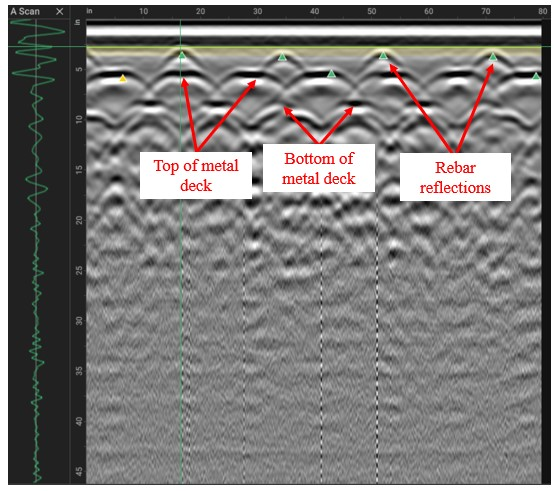
\includegraphics[width=\linewidth]{img/Figure1.jpg}
    \caption{Sample B-Scan GPR Radargram}
    \label{fig:gpr-radargram}
\end{wrapfigure}

% Content
\noindent The continual assessment of concrete is used to guide decisions regarding repairs and maintenance of critical infrastructure. One of the most effective assessment techniques is non-destructive testing (NDT), which allows engineers to gather vital information about the internal condition of a concrete structure without causing physical damage. Among the various NDT methods, ground-penetrating radar (GPR) is particularly valuable for its ability to provide detailed radargram images of concrete structures. However, GPR data is often noisy, making manual interpretation prone to errors. Despite these challenges, recent advancements in computer vision, specifically convolutional neural networks (CNNs), offer a promising solution. CNNs excel at recognizing patterns and features in images, making them ideal for automating the detection of anomalies within GPR data, leading to faster, more accurate assessments of concrete defects. This research project aims to develop a specialized CNN model, ConcreteNet, tailored specifically for the classification and detection of anomalies in GPR radargrams. Furthermore, this research will generate two key outcomes: (1) a neural network architecture optimized for GPR radargram analysis, and (2) a publicly available dataset of GPR scans that will serve as a benchmark for future work. The dataset will be evaluated using state-of-the-art models in image classification, object detection, and weakly supervised object detection (WSOD) to demonstrate its utility as a benchmark. This will generate two academic papers---one focusing on the development and validation of ConcreteNet, and the other on the creation and benchmarking of the dataset against state-of-the-art models.

\subsection{Experimental Plan}
%\textcolor{red}{Implement experimental plan and add figures. reference postdoc thesis that taheri shared with me for a potential experimental plan}
% Rewriting the below in my voice and for clarity
% \noindent In this project, first an appropriate amount of GPR dataset will be acquired and gathered to establish the required dataset for the assessment. This will be done by gathering the historical GPR data which we have acquired over the last few years of our investigation on a concrete bridge deck. In addition, to improve the quality and accuracy of the dateset, as well as providing the larger training dateset, extra data will be acquired from a known structure (in this case the ERB building on campus of GS). Then, \textcolor{red}{please continue with your plans on developing the model and comparing the results as you indicated in the abstract} 

% Content
\noindent The first part of this project will focus on developing the architecture of ConcreteNet. The model will be based on the AlexNet architecture, enhanced using a "Network in Network" approach to capture the subtle and complex features within GPR data. The model will be trained using floor scans from the Georgia Southern Engineering Research Building, chosen for its recent construction date and contemporary design. To simulate structural deformities such as delamination, corrosion, honeycombing, and voids, we will embed these defects into concrete slabs in a controlled laboratory setup, where each type of defect will be introduced at varying depths (from 1 to 5 inches), and add the resulting data to the training set. After the model is trained, it will be validated using existing GPR data provided by the Georgia Department of Transportation, using common metrics such as accuracy, precision, recall, and F1-score to evaluate its performance. For the second part of the project, the training dataset will be benchmarked against state-of-the-art computer vision models to measure cross-dataset model performance and prove the generalization capabilities of each model on the new dataset. The goal is to prove that this dataset poses a significant challenge due to its high intra-class variability, which reflects the diverse and noisy nature of GPR radargrams. We will benchmark this dataset against various cutting-edge models in image classification, object detection, and weakly supervised object detection (WSOD) to demonstrate its difficulty compared to ConcreteNet's performance. For image classification, MobileNet, DenseNet121, and ResNet50 will be tested. For object detection, YOLOv11, RetinaNet, and Faster-RCNN will be evaluated. For WSOD, Wetectron, C-MIL, and PCL will be assessed.

\subsection{Expected Outcomes}
\begin{itemize}
\item Poster presentation at the PCEC and Georgia Southern University-wide Student Research Symposiums
\item Prospective journals: ASNT Journals of Materials Evaluation and Research in Nondestructive Evaluation
\item Prospective presentations: ASNT Research Symposium and ASME-IMECE Conference
\end{itemize}
\newpage

%========================= Budget =========================
\section{Itemized Budget With Justification}
%\noindent This page submits an itemized budget, detailing the allocation of requested funds, and justification for each expense.
% \subsection{Budget and Budget Justification}
\subsection{Budget Breakdown and Justification}
\begin{table}[htbp]
    \centering
    \begin{tabular}{|c|c|c|}
    \hline
    \textbf{Item} & \textbf{Amount} & \textbf{Justification} \\ \hline
    Software and Licensing & \$700 & Essential for neural network training, image processing, and data analysis. \\ \hline
    Materials and Supplies & \$300 & Necessary for data storage and collection hardware; also, experimentation. \\ \hline
    \textbf{Total} & \textbf{\$1,000} \\ \cline{1-2}
    \end{tabular}
\end{table}

% \subsection{Justification}

% \begin{description}
%     \item[Conferences] % Attending conferences is essential for disseminating the research findings and connecting with professionals in fields like AI, non-destructive testing, and infrastructure assessment. The \$100 will cover registration fees for virtual or regional conferences, enabling participation in events such as the ASNT Annual Conference or other AI-related meetings. Presenting the work at these conferences will provide valuable feedback and raise awareness about its potential applications.

%     \item[Software and Licensing] % This project requires specialized software for tasks such as image processing, neural network training, and analyzing GPR data. The allocated \$500 will be used to purchase or renew licenses for software like MATLAB, TensorFlow, and other GPR-specific tools. These tools are crucial for implementing advanced machine learning models and processing complex radargram datasets efficiently.

%     \item[Materials and Supplies] % To support the research, \$400 is allocated for purchasing necessary hardware components and materials, such as external hard drives for data storage and miscellaneous supplies for data collection. Reliable equipment is vital to ensuring smooth operations, secure data management, and backup for large datasets during the project.
% \end{description}

\end{document}
